\documentclass[
  journal=small,
  manuscript=article-type,  % Use a - if you need a space e.g. "research-article"
  year=2022,
  volume=1,
]{cup-journal}

\usepackage{amsmath}
\usepackage[nopatch]{microtype}
\usepackage{booktabs}
\usepackage{caption}
\captionsetup[table]{position=bottom}
\usepackage{hyperref}
\hypersetup{
    colorlinks=true,
    linkcolor=blue,
    filecolor=magenta,      
    urlcolor=cyan,
    pdftitle={Overleaf Example},
    pdfpagemode=FullScreen,
    }

\title{TrashGo: Improve the Human Experience}

\author{In Woo Park}
\affiliation{ICS 691D: Human-Centered AI, University of Hawaii at Manoa}
\email[. Author]{inwoo@hawaii.edu}

\keywords{robotics, autonomous driving, gamification, crowdsourcing} 

\begin{document}
\begin{abstract}
It is our responsibility to properly dispose of our trash. Unfortunately, a great deal of people do not agree with this sentiment. Pollutants on land will eventually make its way into the ocean. We can help stop this process by volunteering our time to pick up trash but this method becomes inefficient once we realize that the problem isn't the trash that we can see, but rather the trash that we can't see. In order to solve this problem, we propose ambitious plan to combine Human-Centered AI methods (i.e., robotics, autonomous driving, gamificaiton, crowdsourcing) in order to develop a cloud-based, real-time, pollutant location database that will motivate individuals to pick up trash. 
\end{abstract}
\vspace*{-2.5em}
\section{Introduction}
At the heart of Hawaiian culture, exists the concept of Malama 'Aina, to care for the land. Although simple, the phrase represents a multitude of concepts when we use it today. Malama 'Aina means to use natural resources wisely, not using more than you require, and replacing the things you take. It means to be aware of endangered species and how our actions have consequences on delicate ecosystems and habitats. Most importantly, Malama 'Aina means to clean up after one-self, being pollution deterrent and not the cause. Being aware of litter, picking up trash, and recycling. Although this seems basic and instinctive, this is not the reality for many people in the State of Hawaii. 

The unfortunate reality is that even if you live far from the coast, the plastic you throw away could make its way into the sea. Plastic can end up in the ocean through the improper disposal of materials. These are but not limited to: improper recycling, littering, or even flushing products down the drain. The State of Hawaii does not deserve this treatment. 

Pollutants on land will eventually make its way into the ocean. We can help stop this process by volunteering our time to dispose of these pollutants ourselves. Finding volunteers to pick up trash is generally not the issue (i.e., 808 Cleanups, Sustainable Coastlines Hawaii, Hawaii Wildlife Fund). The issue is that most litter are pollutants that we don't see. It's easy to dispose of pollutants when they are piled in abundance, but difficult when exist by themselves. Single pieces of plastic, paper, or aluminum are easily missed and often forgotten for long periods of time. Eventually these pollutants will end up in the ocean. Therefore, how can we make it easier to find these pollutants? What can we do to make the volunteers job easier? Introducing TrashGO.

\section{An Ambitious Plan}
TrashGO is a concept design that will combine Robotics, Autonomous Driving, Crowd-sourcing, and Gamification methods to develop a cloud-based, real-time pollutant location database that will motivate individuals to pick up trash.

\section{Research Design and Methods}
There are six aims that need to be accomplished for TrashGO to be successful. Each aim is a challenge in their own right as they address the four human-centered AI methods that will be used to build the TrashGO Architecture. Using a combination of focus, commitment, and sheer will, this network of ultimate trash robots will take over the world.

\begin{figure*}[h!]
    %\centering
    \hspace*{-.75cm}
    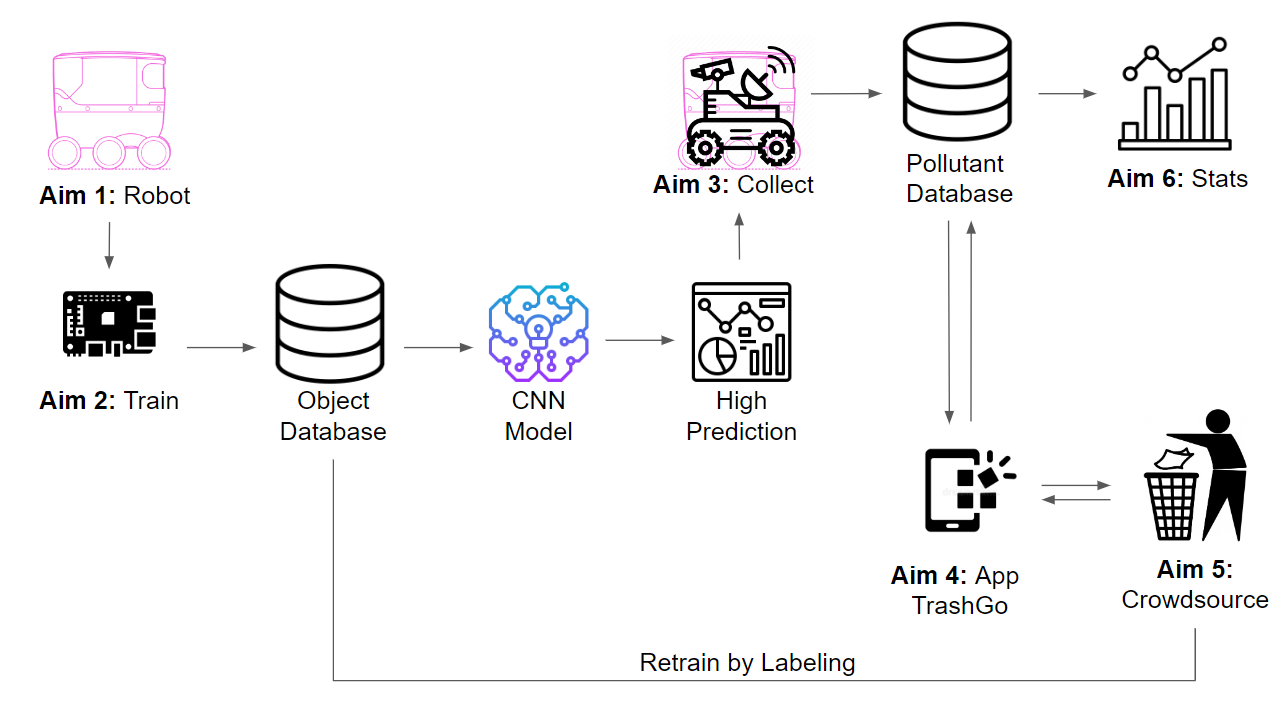
\includegraphics[scale = .4]{aims.png}
    \caption{TrashGO Architecture}
    \label{trash_architecture}
\end{figure*}
\vspace*{-2.0em}
\subsection{Aim 1: Designing a Robot}

On Janurary 23, 2019, Amazon Scout debuted as a six wheeled delivery robot. Amazon Scout robots are fully electric, can carry a payload of 50lbs (23 kg) and have a maximum speed of 15 mph (Amazon Scout Dimensions). Although Amazon themselves haven't disclosed how Amazon Scout works,if it's anything like Starship Technologies, an Amazon competitor for autonomous delivery robots, Amazon Scout most likely uses a combination of GPS, cameras, and neural networks for object detection to traverse the world. However, on October 6, 2022, Amazon stopped field tests and scaled back work on Amazon Scout (Soper 2022).
\\\\\textbf{Method}\\
Develop an autonomous robot by using a design similar to those from Amazon Scout or Starship technologies or by re-purposing Amazon Scout delivery robots. For our scenario, let us assume we have acquired and re-purposed autonomous Amazon Scouts. 

The robot most likely accepts two addresses, a destination address (delivery address) and a source address (warehouse address). Change the route a robot takes by arbitrarily adding more destination addresses to visit, allowing the robot to traverse a neighborhood in a rectangular pattern, and eventually returning to the source address. 

In case we don't receive the robot with Amazon's Object Detection model included (Tanel 2018), we can load a pre-trained model into TrashGO Scout. The pre-trained, transfer learning object detection model of choice is YOLO, or the 'You Only Look Once' model (Subhash 2019). YOLO uses features from the entire image to predict each bounding box and their classes simultaneously (Sigel 2019). YOLO is able to recognize where and what objects are within a given image by running the image once through the CNN (Singh 2022). For our purposes, we will use this object detection model to avoid collisions between our robots and the real world (QuinnRadich). The pre-trained model weights has been trained detect 80 classes (categories) for everyday objects (i.e., bus, person, sandwich, etc)(VOC, PASCAL Visual Object Classes Challenge). 

Eventually, we will want our own dataset with custom classes (i.e., Trash\_plastic, Trash\_cans, Trash\_paper, Trash\_cardboard) (Aim 2). Later we will discuss how we can build this dataset by using crowdsourcing methods to label data (Aim 5). 

The robot will travel at a reasonable speed (i.e. 2mph) where adequate time will be available to avoid collision. The robot will not have to cross the street in our scenario and will traverse the world in mostly straight paths on the sidewalk only. 
\\\\\textbf{Evaluation}\\
Evaluate the design of the robot by allowing the robot to autonomously drive through a pre-defined path whilst successfully avoiding collision between itself and other objects. The pre-defined paths will gradually increase in difficulty after each successful evaluation. Evaluation will be split into five different tests. 

The first test will be an open world scenario. Let the robot move from point A to point B unobstructed in a open environment (i.e., empty parking lot). If the robot successfully moves from its source address to a destination address within a six feet margin of error to account for GPS inaccuracy, the robot has passed the first evaluation. 

The second evaluation will shorten the size of the robots world by reducing the open environment to the width of five feet, the average width of a sidewalk in the United States. Collision has not been thoroughly tested so we will reuse the empty parking lot and paint a outline of a sidewalk to the length of thirty feet. The robot will pass this evaluation if it moves from point A to point B within a margin of error of six feet to account for GPS inaccuracy, and if the robot stays within the painted line during its travel across the lot. 

The third evaluation will repeat the same scenario of the previous evaluation but now include obstacles for the robot to avoid. These obstacles will be objects that the pre-trained object detection model will recognize in addition to general collision detection methods (i.e., pedestrians, street signs, cars, bicycles). The robot will pass this evaluation if it moves from point A to point B within a margin of error of six feet, if the robot stays within the painted line during its travel across the lot, and if it successfully completes the travel by avoiding collision with obstacles. We should expect a collision rate of zero, or no collisions at all. We should expect that all collision faults are due to exterior forces acting on our robot. 

The fourth evaluation will repeat evaluation three methods but now add left and right turns for the robot to traverse, keeping all settings the same (i.e., street width, destination margin of error, typical obstacles, collision rate).

The fifth evaluation will repeat the fourth evaluation method but in a real world scenario. We will conduct fifty tests across a random selection of districts in the State of Hawaii based on street length, giving priority to streets with longer lengths.  
The robot will perform better in a scenario similar to it's training environment, therefore, let us test the robot on streets with long straights as the robot will not be programmed to cross the street to reduce over complication. 

\subsection{Aim 2: Training an Object Detection Model}
\textbf{Method}\\
Similarly to the second half of Aim 1, we will need to implement transfer learning using the object detection model, YOLO, but now on a custom dataset. Instead of adding more classes to Aim 1's model for trash related objects, we have decided to have a second object detection model specifically for pollutants. The reason for this separation is to see if we can have the pollutant model be extremely successful in detecting a few classes (i.e., 10) instead of mediocre at detecting many classes (i.e., 80+. Fortunately, we can take inspiration from Maarten Sukel (Sukel 2019), a data scientist who has had a similar problem to ours by developing a garbage object detection model using PyTorch and YOLOv3 (Maarten 2019). His pre-trained weights were for four classes: cardboard, garbage bags, containers, and cigarettes. If we want to add more classes (i.e., paper, plastics, cans), we will need to build upon his pre-trained weights by collecting more images for those objects and labeling them. Let us collect 333.33 images for paper, plastics, and cans, in the context of pollution for a total of 1000 images and label them. Let us collect 200 more images of paper, plastics, and cans in the context of pollution from areas where we would deploy TrashGO Scouts. We need to make sure that each image we insert into the original dataset is standardized to the same image format, resolution, and how the image is labeled. 
\\\\\textbf{Evaluation}\\
The initial 1000 images will be split 80/20 for training set and validation set. The 200 additional images from areas where we would deploy TrashGO Scouts will be used as our clean test set. The model will most likely have low precision ($<$ 0.50) and high recall as the pre-trained model we are building from reported these results. There reasoning for this was that real world objects share common shapes in addition to a lack of variety of images in the dataset. We should be able to increase precision by adding more images that contain no pollutants in addition to images with pollutants. An acceptable precision will be $> 0.60$ precision for the initial deployment. We consider this an acceptable baseline because our initial deployment of TrashGO markers will contain many false positives regardless of how well the object detection model has trained. Our initial test set will be pictures of pollutants in an entirely new environment (i.e., Downtown Honolulu, Kapolei), therefore, it is more likely that submitting images from these new environments into our training set will help increase our precision score over time. Luckily we can solve this issue through Aim 5, crowdsourcing the work. When our app initially releases, we can let the users passively participate and label as much markers as they can. This data will be collected and sent back to the dataset in order to re-train the model. Through this process, we can gradually build upon the database with new images and labels each day. 

In addition to observing an increase in our models precision score, we can use the data gathered from Aim 5 to determine our models performance over time. We can user label data from users to determine the actual false positive rate of model as each image that is captured and labeled is treated as part of the test set then back into the training set. Users labeling markers may give us insight on our models behavior and whether we are overfiting or underfitting to the training set. 

\subsection{Aim 3: Pollutant Location Database}
\textbf{Method}\\
Develop a cloud-based, real-time pollutant location database using Amazon Web Services DynamoDB. DynamoDB is a non-relational key-value pair database that is highly partitionable and allows for horizontal scaling of attributes. 

Crowdsource data collection by deploying a series of TrashGO robots to traverse independent sections of a neighborhood, using its object detection model to detect for pollutants. The robot will be equipped with an on-board 4G LTE GPS tracker for accurate lat-long coordinates of its current location. Once a robot has decided an object it has encountered is trash, it will internally store an ID of the object, the objects type, confidence score, time of detection, geographical latitude and longitude, and an image of the object (Figure 2). The ID of the object will contain an abbreviated version of a neighborhoods name in addition to the count (i.e., DT\_1 is Downtown 1, KLH\_1 is Kalihi 1).

\begin{table}[h!]
    \centering
        %\caption{Caption}
        %\label{tab:my_label}
    \begin{tabular}{ | l | l | l | p{1.5cm} | l | l | l |}
    \hline
    ID & Type & CScore & Time & Latitude & Longitude & S3ID \\ \hline
    DT\_1 & Paper & .63 & 11/22/2022 05:53:21 & 27.2046 N & 77.4977 E & ../DT/DT\_1.png\\ \hline
    DT\_2 & Can & .67 & 11/22/2022 05:54:02 & 27.6246 N & 77.5012 E & ../DT/DT\_2.png\\\hline
    DT\_3 & Plastic & .88 & 11/22/2022 05:54:27 & 27.8086 N & 77.5022 E & ../DT/DT\_3.png\\\hline
    KLH\_1 & Cardboard & .65 & 11/22/2022 05:30:59 & 30.8746 N & 80.5221 E & ../KLH/KLH\_1.png\\
    \hline
    \end{tabular}
    \caption{DynamoDB Key-Value Table}
    \label{table:my_label}
\end{table}

Once the robot returns to its source location, it will be connected to a secure network where it can upload its internal key-value storage to DynamoDB through the AWS Mobile SDK (Aim 4). DynamoDB should not hold the actual image as it is a key-value database, therefore, when the robot uploads to our database, it will trigger a Lambda function to send the images to an S3 bucket. Once placed in the S3 bucket, a final Lambda function will trigger to return image S3 object identifier values back to DynamoDB to be stored in the S3ID column. 

\begin{figure*}[h!]
    %\centering
    \hspace*{-.75cm}
    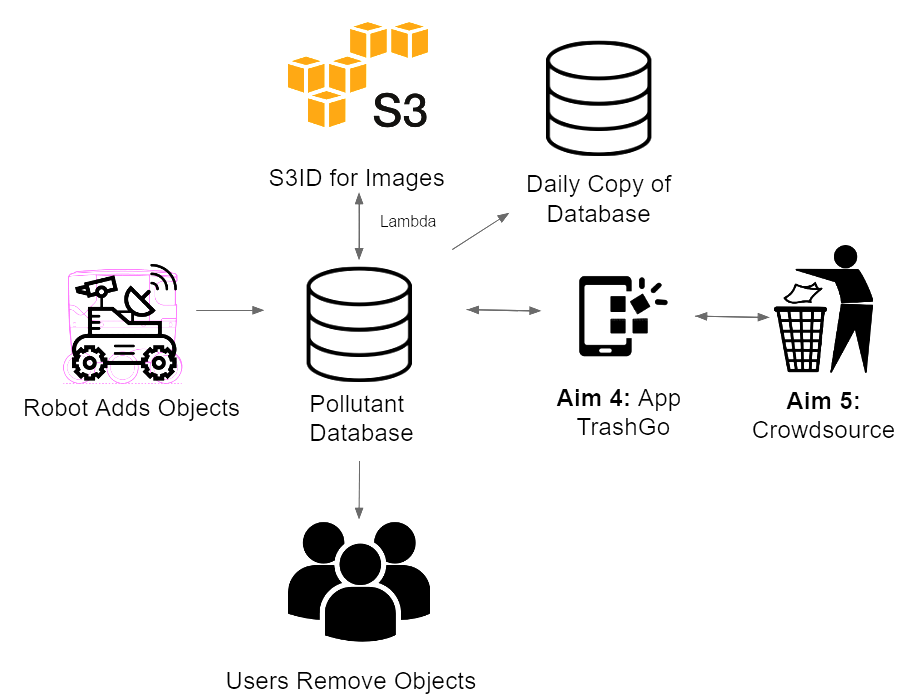
\includegraphics[scale = .35]{DyanamoS3sync.png}
    \caption{DynamoDB, S3, TrashGO Architecture}
    \label{trash_db}
\end{figure*}

Our DynamoDB table will grow and shrink dynamically as pollutants are added by robots or removed by users, therefore, we do not have predictable application traffic or capacity requirements to control costs. We will opt for on-demand capacity mode for DynamoDB. Finally, let us create a master copy of the database for each day so we can use the data gathered to re-train our object detection model (Aim 2). 
\\\\\textbf{Evaluation}\\
All instances that exist within our pollutant location database will have a confidence score provided by our YOLO object detection model. We can introduce human-in-the-loop machine learning by crowdsourcing (Aim 5) the labeling of pollutant objects within our database through a mobile app (Aim 4). A new database of pollutant images will be generated each day which will be labeled by humans to be sent back to model (Aim 2) for continuous retraining. We can evaluate the improvement of our model by randomly selecting pollutants and their confidence scores from a previous day's database, passing the same image to the newest model, and compare the change in confidence scores over time. After some time, the database should contain more unique, labeled, real-world objects than the number of objects from the original dataset that was used to train the model. 

We know that our database is configured properly if we can 
migrate marker data from the robots to DynamoDB, store images on S3, have a hot backup of database available, and if DynamoDB is set to on-demand due to unpredictable activity. 

\subsection{Aim 4: The Mobile App}
\textbf{Method}\\
Develop a mobile app using AWS Amplify to gamify the human-in-the-loop labeling of pollutants and to provide users the location of pollutants (Engdahl 2017). The mobile app will use Google Maps API to display the GPS location of the user and the location of nearby pollutants by translating lat-long data as markers on the map (Figure 3). Each marker will synchronize once every ten minutes with DynamoDB to check if the object has been crowdsourced by another user (Aim 5). All metadata will be visible to the user on the app (Figure 4). Users will be able to approach each marker and interact with them through their device. They will be granted an option to label the marker or to label and dispose of the marker. Users will also be able to view the metadata per marker (Figure 5).  
\begin{figure*}[h!]
    \centering
    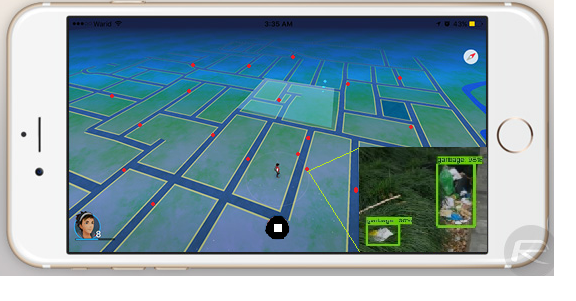
\includegraphics[scale = .8]{phoneGO.png}
    \caption{TrashGO Gamification: Playing}
    \label{trash_gameplay}
\end{figure*}
\vspace*{-1.5em}
\\\\\textbf{Evaluation}\\
To evaluate the mobile application, it must successfully report the GPS coordinates of every pollutant marker. Each user has the ability to update the database by interacting with a pollutant marker on the mobile app (i.e., disposing of trash and marking the trash disposed of). Therefore, by setting a pollutant marker as complete, AWS Amplify will trigger an AWS Lambda Function to remove an item from the DynamoDB table by Object ID (i.e., DT\_1). In order to reduce the cost of running this application, each device will check if three criteria have been met before sending update data to DynamoDB.

\begin{itemize}
    \item (1) Is the user within reasonable proximity to the pollutant?
    \item (2) Has the user labeled the object?
    \item (3) Has the user uploaded a confirmation image of the pollutant? 
\end{itemize}

Each device that attempts to contact DynamoDB will only increase the resource cost of the application as well as the cost per database update. These criteria will deter users from sending false marker reports and reduce resource cost of update the main database. To handle passive updates from a user (Aim 5), let the user store the labeled object data on their device. Let all devices send a master update from each device to the server once a day at some arbitrary time.

\begin{itemize}
    \item (4) Exclusive OR: Is the current time 00:00:00?
\end{itemize}

Each device will send information to DynamoDB if they meet some pre-defined criteria. DynamoDB will update the table by removing objects correlated to markers that have been flagged as disposed. Each device will then pull the most recent version of the pollutant database. The amount of markers displayed on the mobile app will decrease throughout the day. A perfect day is when all markers are removed from your neighborhood, and a successful day is when more than half of markers are removed. 

\begin{figure*}[h!]
    \centering
    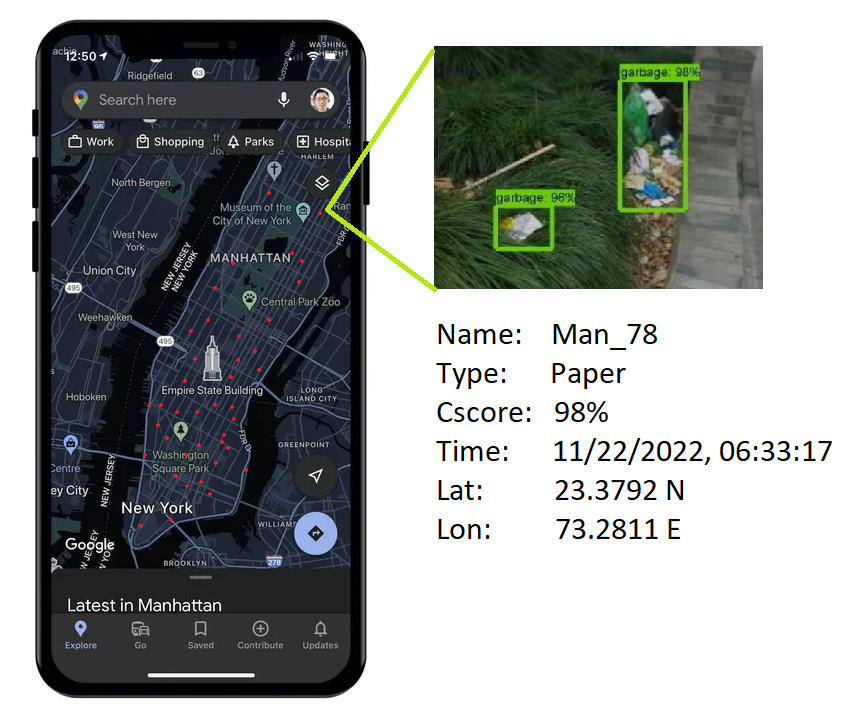
\includegraphics[scale = .5]{appBird.png}
    \caption{TrashGO Gamification: Labeling}
    \label{trash_game}
\end{figure*}
\vspace*{-1.5em}
\subsection{Aim 5: Crowdsourcing the Work}
\textbf{Method}\\
Users may contribute to TrashGO either passively or actively. 

Passively: Users who are not able to assist in the disposal of pollutants may contribute by labeling objects. Regardless of TrashGO's confidence score, users may virtually visit each marker and provide a label for each pollutant (classification and type). Users may also be asked to label other things if most markers of the day have already been labeled. (i.e., reCAPTCHA).

Actively: Users who are able to assist in the disposal of pollutants may contribute by physically traveling to each marker, labeling the marker, flagging the marker as complete, and finally disposing of the pollutant properly. Users will be able to add their own markers in future iterations of TrashGO.
\\\\\textbf{Evaluation}\\
Allowing a user to label a marker and accepting that as the ground truth will give too much power to the user. There is a possibility that malicious users may incorrectly label multiple markers. Therefore, let us use user labeling data as votes for an internal balloting system, where the majority of votes represent an objects categorical ground truth with an arbitrary value (i.e., 100) as the minimum number of votes required for a marker to update its label. Long time users of the app will eventually be considered more trust worthy based on their total contribution to TrashGO crowdsourcing, allowing their vote to have more weight when labeling a marker. Eventually this will allow our algorithm to use a fewer number of votes to update a markers label (i.e., 100 regular user versus 4 trusted users).

\section{Conclusion}
Obviously, our solution for a cleaner world is a novel but unorthodox approach. Each independent component requires an equal amount of time, resource, and effort for the project to succeed. Not only does each aim have to be carefully designed and deployed, but also each aim must integrate with each other. Our proposal started with robotics, or designing a robot that will act as data collector. The robot will be given the ability to travel and avoid colliding with the world through a pre-trained, transfer learning object detection model called YOLO. When we believe our model is ready for deployment, we will let the robot traverse the world, capturing images and locations of pollutants it can find. Once captured, we will upload this data to our pollutant database hosted in the cloud, share that data with our mobile application, and allow users to interact with the data through active or passive methods. Finally, new images of pollutants found by the robot will be sent back to our model for re-training. We hope that our pollutant location database will motivate individuals to pick up trash. A large problem with this type of volunteer work is time and efficiency. Hopefully we can alleviate this problem with our database which will mostly be used as a trash map. 

If we were to revisit the design board for this project, we will provide more information for Aim 6, useful statistics. We did not have a write a up for this section as it requires to have actual real world data in order to perform data analytics. We can only imagine the useful information we can find through our database (i.e., trash per square feet between different city districts, ranked by economical or social status of their communities. Is Kalihi more likely to have a higher count of pollutants than Manoa? What is the count of trash associated with a districts political party?) 

In addition, we would also cover project funding. Our assumption for Aim 1 was that Amazon would agree to re-purpose their Amazon Scout robots for our proposal, but what motivation does Amazon have to join our mission? One  idea we had was to give each robot ownership of their trash. In other words, once a pollutant is marked, we will keep track of the robot that submitted the mark, and sum the average weight of each trash that has been disposed of by a user. At the end of the year, we will have some statistic showing how much pounds of trash were removed with the help of each robot. This statistic can be used by Amazon to support their 2019 climate pledge to reach net-zero carbon emissions by 2040. In addition to using Amazon's proprietary robot design, we will also be using AWS to build our network infrastructure to operate TrashGO. We believe these factors may convince Amazon to consider our proposal. 

\newpage
\begin{thebibliography}{9}

\bibitem{Journal}
Amazon Dynamodb: How It Works - Amazon Dynamodb. https://tinyurl.com/2ue32d8h.

\bibitem{Journal2}
“Amazon Scout Dimensions; Drawings.” RSS, https://tinyurl.com/ycrswsf3.

\bibitem{Journal3}
D, Subhash. “Best Pre-Trained Models for Object Detection in Machine Learning.” IT4nextgen, 20 Aug. 2019, https://tinyurl.com/3k4we9xe.

\bibitem{Journal4}
Engdahl, Sylvia. “Using Amazon DynamoDB Document API with the AWS Mobile SDK for Android – Part 2.” Amazon, Greenhaven Press/Gale, 2008, https://tinyurl.com/6929f59h.

\bibitem{Journal5}
“GPS Logger.” Including Gyro / Tilt / Compass; Accelerometer - Aaronia AG, https://tinyurl.com/4x5tadeh.

\bibitem{Journal6}
Hui, Jonathan. “Real-Time Object Detection with Yolo, yolov2 and Now yolov3.” Medium, Medium, 6 Sept. 2022, https://tinyurl.com/3w9n5rt7. 

\bibitem{Journal7}
Maarten Sukel. “Garbage Object Detection Using PYTORCH and yolov3.” Medium, Maarten Sukel, 10 Oct. 2019, https://tinyurl.com/2p8tvfup. 

\bibitem{Journal8}
Parnamaa, Tanel. “How Neural Networks Power Robots at Starship.” Medium, Starship Technologies, 28 Nov. 2018, https://tinyurl.com/yc7yj3zy. 

\bibitem{Journal9}
QuinnRadich. “Train Your ML Model with Tensorflow.” Train Your ML Model with TensorFlow | Microsoft Learn, https://tinyurl.com/dru2r22z. 

\bibitem{Journal10}
Singh, Sumit. “Guide on Object Detection; Its Use in Self-Driving Cars.” Labellerr, Labellerr, 11 Oct. 2022, https://tinyurl.com/5n7vwavy. 

\bibitem{Journal11}
Soper, Taylor. “Amazon Stops Field Tests and Scales Back Work on Scout, Its Home Delivery Robot Program.” GeekWire, 7 Oct. 2022, https://tinyurl.com/muymz3zb. 

\bibitem{Journal12}
Sukel, Maarten. “Pytorch Implementation of an Urban Object Detection Model.” GitHub, 2019, https://tinyurl.com/yedys8ep. 

\bibitem{Journal13}
“VOC. Tensorflow Datasets.” TensorFlow, https://tinyurl.com/ypwu5ywc. 

\bibitem{Journal14}
Wen, Sigil. “Object Detection with YOLO: Bringing Vision to Self-Driving Cars.” Medium, Towards Data Science, 11 Dec. 2019, https://tinyurl.com/y873zkxa. 

\end{thebibliography}

\end{document}
